\documentclass{article}
\usepackage[utf8]{inputenc}
\usepackage{ctex}
\usepackage{amsmath}
\usepackage{amsfonts}
\usepackage{amssymb}
\usepackage{graphicx}
\usepackage{amsthm}
\usepackage{cite}
\usepackage{float}
\usepackage{fontsize}
\title{Mandelbrot 集合图像绘制报告}
\author{lpr}
\date{2025.3.14}

\begin{document}

\maketitle

\section{Mandelbrot 集介绍}

$\textbf{Mandelbrot 集}$ 对于迭代公式 $z_{n+1} = z_n + c$,如果复数 $c$ 经过无限次迭代,其模仍然有限,则 $c$ 包含于 Mandelbrot 集合。 

\section{程序使用到的定理以及公式}

$\textbf{定理 1}$  $\forall c \in \mathrm{Mandelbrot} ,\forall n \in \mathbf{N^*}, |z_n| < 2$  

$\textbf{公式 1}$  ${z_{n+1}}' = 2z_n{z_n}' + 1$

$\textbf{公式 2 距离估计公式}$  $\mathrm{Dis}(z_n) = \frac{\sqrt{ \frac{|z_n|}{|z_n|'} }}  {2\ln{z_n}}$,其中 $z_0' = 0$

\section{程序算法简述}

{\footnotesize$\textbf{请注意分清 “点” 和 “像素点” 的区别}$}

\begin{description}
    \item[初始化] 将 config.json 中的初始数据读入,设定图片分辨率为 $$\frac{x_{\max} - x_{\min}}{10^{resLevel}} \cdot \frac{y_{\max}-y_{\min}}{10^{resLevel}}$$,然后初始化opencv的画布。
    \item[计算点距离] 将 $x_{\min}$ 到 $x_{\max}$ 映射到整数,每一列(此处列指的是像素的一列)用 Intel TBB 的开源库进行并行计算。每一行再从 $y_{\min}$ 到 $y_{\max}$ 循环。得到当前像素点对应具体点坐标后
                     以该点在复平面上对应的复数 $c$ 计算该点到 Mandelbrot 集合边界的距离(见公式 2)。   
    \item[绘制] 得到当前点到 Mandelbrot 集合边界距离,如果点在 Mandelbrot 集合之内(距离是负的),对应像素点的灰度 grey 为 255。
                如果此具体点在外面,则由边界距离计算该点所代表的范围中,在 Mandelbrot 集合外面的点的估计密度 density。对应像素点灰度 grey 为 255*density
    \item[监听键盘事件] 使用 opencv 的 waitKey(int) 函数监听键盘事件,通过键盘的输入实时改变设定的参数并重新计算和绘制。            
\end{description}


\hrule
\vspace{3em}
{\footnotesize
$\textbf{密度的估计}$ 计算一个像素点表示的正方形的区域面积。即:$$S = \frac{(x_{\max} - x_{\min}) \cdot (y_{\max}-y_{\min})}{\mathrm{weight} \cdot \mathrm{height}}$$

                     我们估计,以这个正方形区域的中心点为圆点,即我们用于计算迭代的具体的点,以边界距离为半径的圆内的所有点,都在 Mandelbrot 集合内,圆外所有点,都不在集合内。

                     因此,我们得到密度估计公式:$$\mathrm{Density} = \frac{\pi \mathrm{r}^2}{S}$$

                     此处 $r$ 即边界距离
}

\begin{figure}[H]
    \centering
    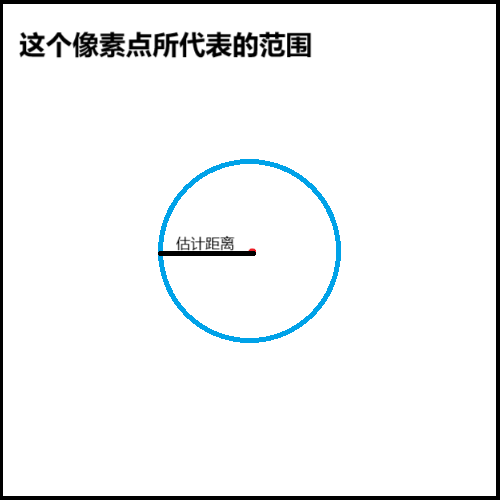
\includegraphics[scale=0.5]{pic.png}
\end{figure}

\end{document}